\chapter{Entwicklung der User Experience mit Verwendung des Google Design Sprints}

Die Entwicklung eines nutzerfreundlichen und effektiven UX-Design-Konzepts zur Abstimmung von Schichtwechseln wurde mithilfe des GDS realisiert. Ursprünglich wurde der GDS für einen Zeitraum von fünf Tagen entwickelt, um schnell Lösungen für komplexe Probleme zu finden und neue Ideen zu testen. In diesem Projekt wurde der GDS aufgrund der Durchführung durch eine Einzelperson angepasst.

Die Phasen 4 und 5 des GDS, die normalerweise die Entwicklung eines Prototypen und das Testen umfassen, wurden modifiziert. Stattdessen wurde ein umfangreiches Bedienungskonzept entwickelt, auf dessen Grundlage eine Nutzerumfrage durchgeführt wurde (siehe Kapitel~\ref{chap:nutzerumfrage}) .
Die Ergebnisse dieser Umfrage wurden anschließend genutzt, um den Prototypen zu erstellen.
%(siehe Kapitel~\ref{chap:prototyp}) 

\section{Phase 1: Verstehen und Definieren}
In der ersten Phase werden die benötigten Informationen gesammelt und analysiert, um das Problem umfassend zu verstehen und klar zu definieren. Die Problemstellung und Zielsetzung wurden bereits in der Einleitung ausführlich behandelt, daher wird in diesem Kapitel direkt auf die praktische Anwendung der nächsten Phasen eingegangen.

\section{Phase 2 und 3: Skizzieren und Auswahl der Idee}
In der Skizzieren Phase beginnt der Prozess der Designerstellung. Hierbei wurden sich zunächst die benötigten Seiten überlegt, um die benötigten Aufgaben und Anforderungen zu erfüllen. Dazu gehört eine Übersichtsseite auf der alle aktuellen Tauschangebote stehen und worüber der Nutzer zu allen weiteren Seiten gelangt, z.B. die zum Hinzufügen und zum Annehmen eines Tauschangebots, sowie eine Seite, auf der der Nutzer seine angenommen Schichten sehen kann und individuelle Einstellungen vornehmen kann. 

Die erste Version der Übersichtsseite war zunächst für einen Desktop ausgelegt (siehe Abbildung \ref{Version1_Desktop}). 

\begin{figure}[h]
    \centering
    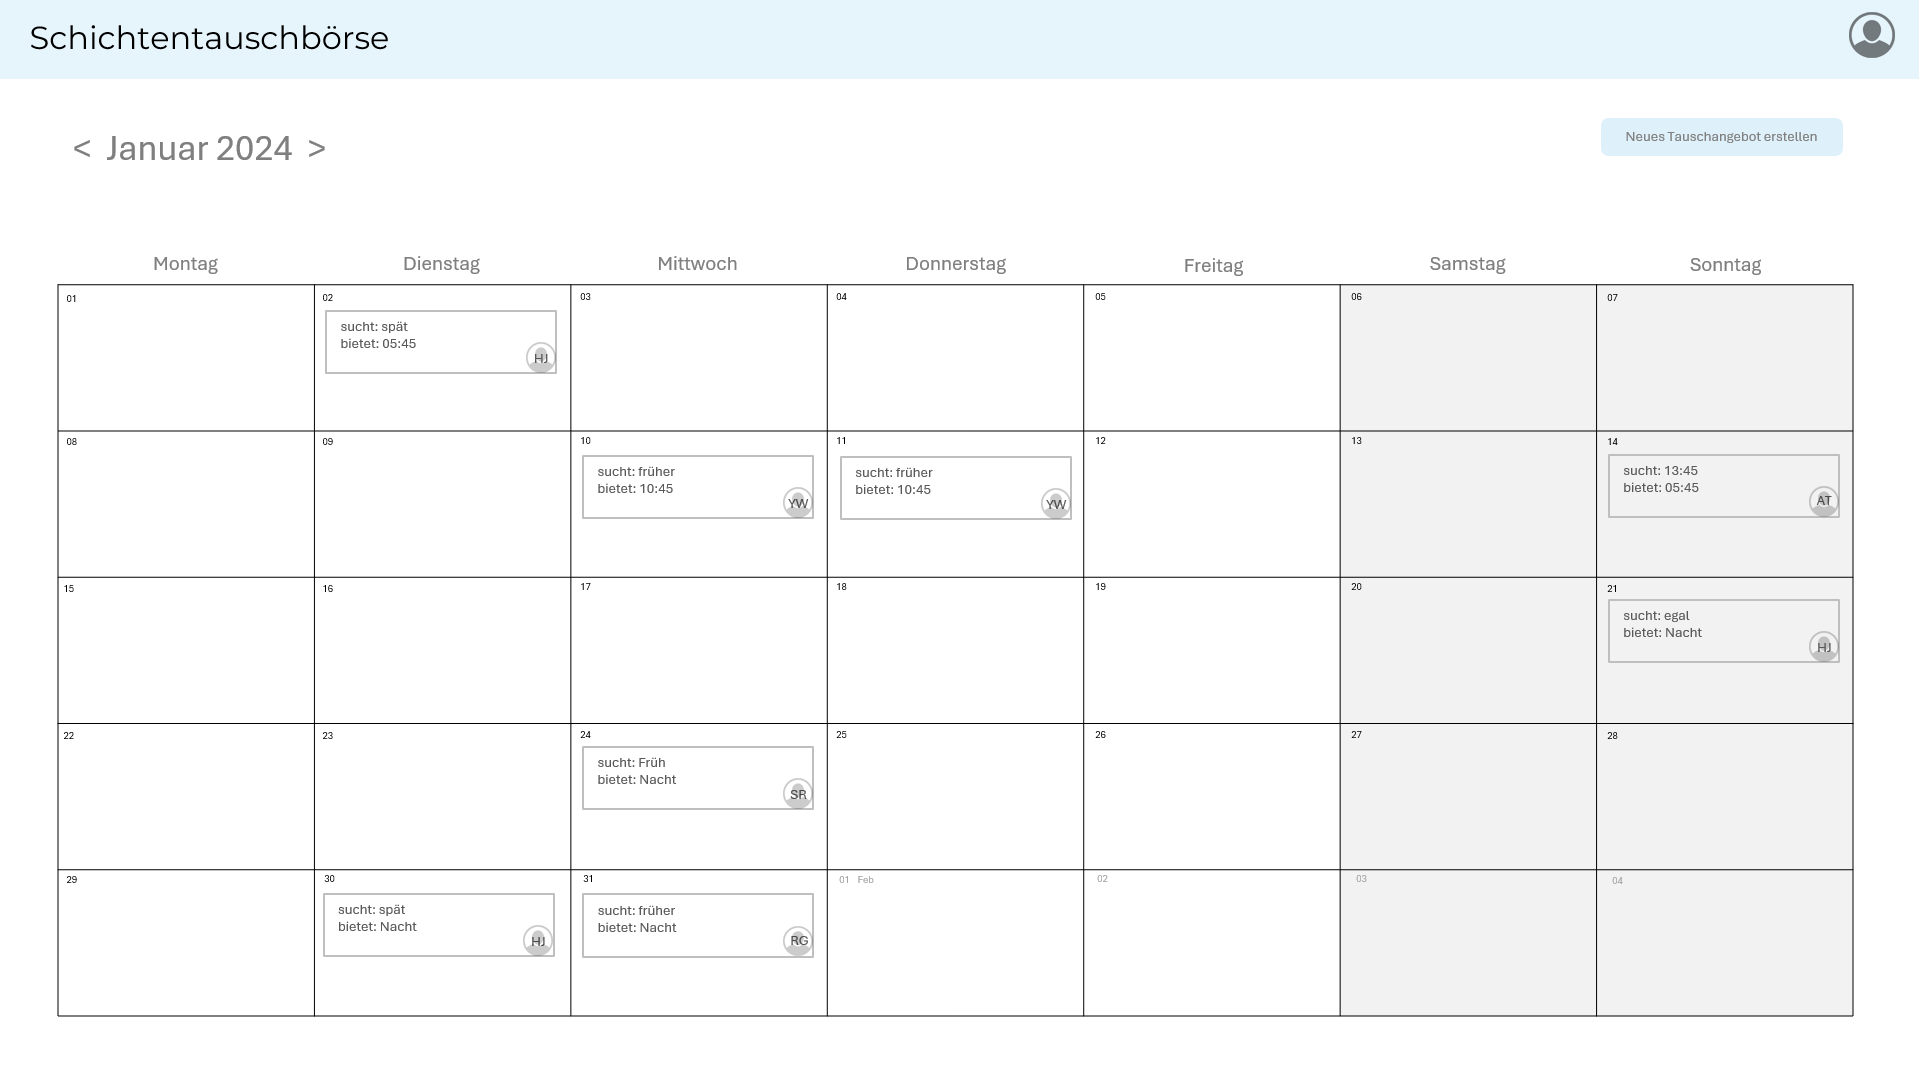
\includegraphics[clip,width=0.9\linewidth]{images/Version1_Desktop.png}
    \caption[Erste Version der Übersichtsseite für den Desktop]{Erste Version der Übersichtsseite für den Desktop}
    \label{Version1_Desktop}
\end{figure}

Im oberen Bereich der Seite befindet sich der Header. 
Links darunter hat der Nutzer die Möglichkeit zwischen den Monaten zu navigieren. 
Rechts unter dem Header befindet sich “Neues Tauschangebot erstellen” Button, mit dem Nutzer neue Tauschangebote erstellen können. 
Zentral auf der Seite ist der Kalender des aktuellen Monats groß dargestellt, die Wochentage sind darüber ausgeschrieben.

Bei der Übertragung des Designs in die Handy-Version wurden einige Schwachstellen identifiziert. Die Darstellung des Desktop-Designs auf dem Handy führt dazu, dass die Schrift aufgrund der kleinen Größe schlecht lesbar war (siehe Abbildung \ref{Version12_Handy}). 

\begin{figure}[h]
    \centering
    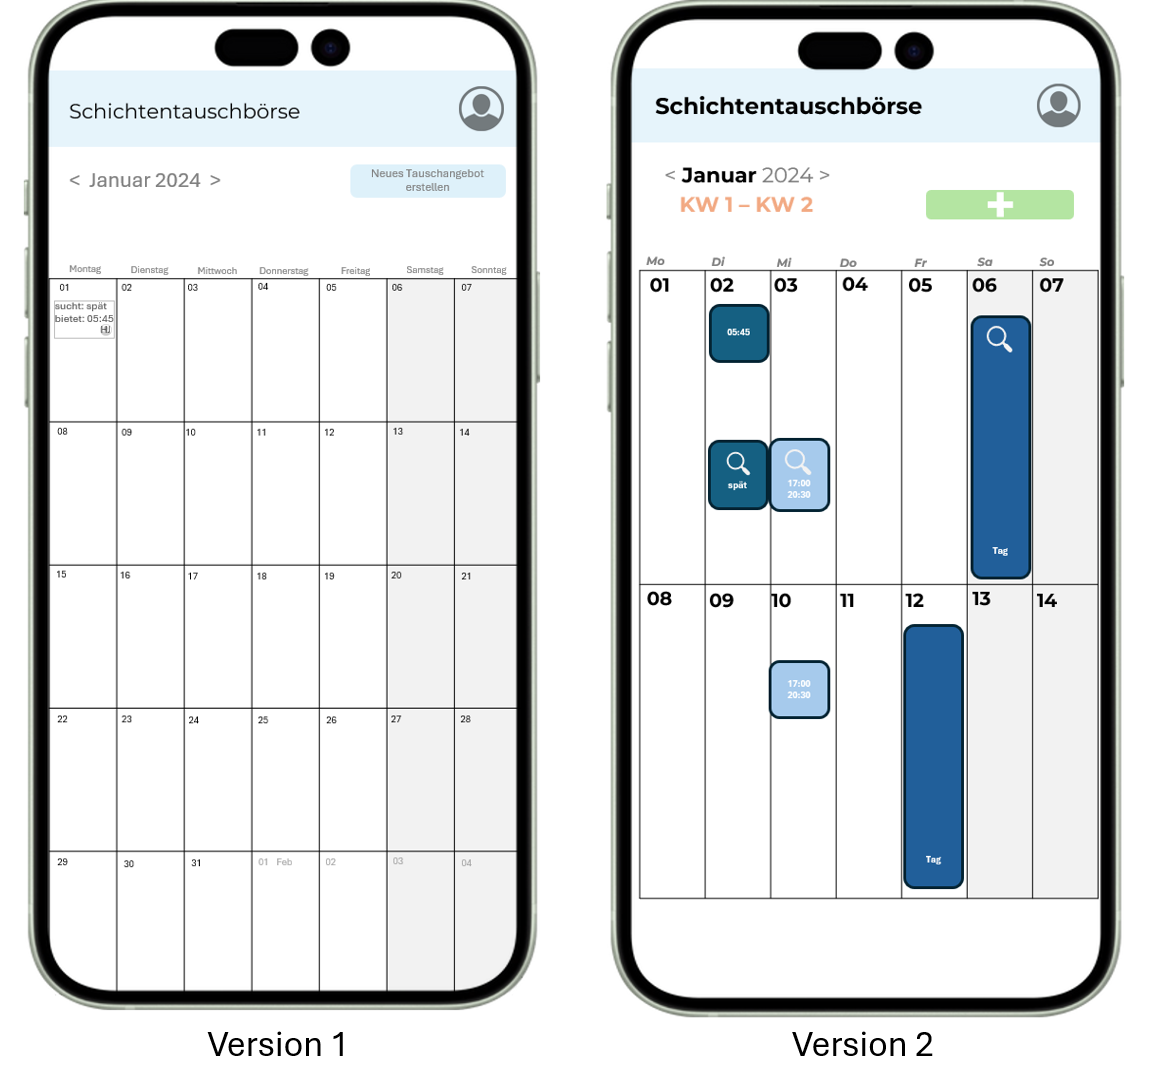
\includegraphics[clip,width=0.75\linewidth]{images/Version12_Handy.png}
    \caption[Erste und zweite Version der Übersichtsseite für das Handy]{Erste und zweite Version der Übersichtsseite für das Handy}
    \label{Version12_Handy}
\end{figure}

Da die meisten Nutzer die App wahrscheinlich auf dem Handy verwenden möchten, wurde das Design in Version 2 entsprechend angepasst.

Um in der Kalenderübersicht die Tauschanfragen gut lesbar und nutzerfreundlich darzustellen, werden statt fünf Wochen nur noch zwei Wochen angezeigt (siehe Version 2 in Abbildung \ref{Version12_Handy}). 
Aufgrund der schmaleren Handybildschirme wird ein Teil der Wörter durch Piktogramme ersetzt, z.B. wurde beim “Neues Tauschangebot erstellen” Button der Text durch ein Plus ersetzt. Dadurch wird Platz gespart und die Funktion wird klarer erkannt. 
Außerdem werden die Wochentage nicht mehr ausgeschrieben. Eine weitere Änderung ist, dass die Schichten in den gesuchten/gebotenen Zeit Blöcken am Tag abgebildet (siehe Version 2 in Abbildung \ref{Version12_Handy}).

Allerdings wurde festgestellt, dass der Kalender unübersichtlich wird, wenn mehrere Tauschangebote an einem Tag sind oder wenn welche zum gleichen Zeitpunkt angefragt werden. 
Deswegen wird eine weitere Version erstellt, in der die Schichten nicht mehr nach dem Zeitpunkt sortiert sind, sondern in einem Block organisiert, was eine bessere Übersicht ermöglicht (siehe Abbildung \ref{Version3_Handy}).

\begin{figure}[h]
    \centering
    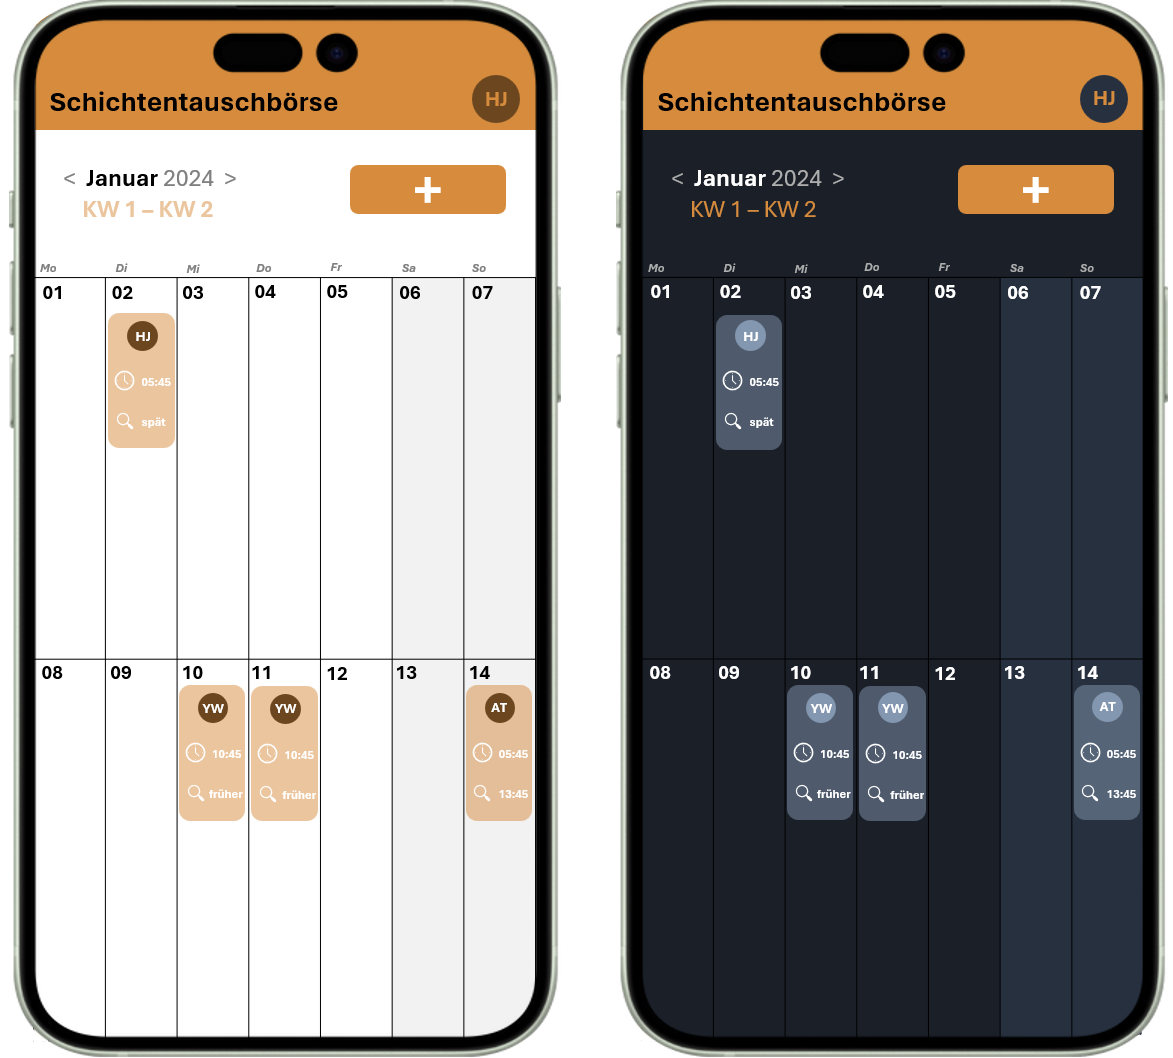
\includegraphics[clip,width=0.75\linewidth]{images/Version3_Handy.png}
    \caption[Dritte Version der Übersichtsseite für das Handy, im Light Mode und Dark Mode]{Dritte Version der Übersichtsseite für das Handy, im Light Mode und Dark Mode}
    \label{Version3_Handy}
\end{figure}

Des weiteren wurde die Hauptfarbe von einem hellen Blau zu einem Orange gewechselt, welches wärmer und aktiver wirkt. Da der Dark Mode in den letzten Jahren stark an Popularität zugenommen hat \cite{diva2020darkmode} wird für die Anwendung auch ein Farbkonzept erstellt (siehe Dark Mode in Abbildung \ref{Version3_Handy}). 

Für die dritte Version wurde sich letztendlich entschieden. Darauf aufbauend wurden die weiteren Seiten der Anwendung im Light Mode gestaltet.

\section{Phase 4: Entwicklung des Bedienungskonzepts}
\label{sec:bedienungskonzept}
Um den Nutzern eine bessere Vorstellung von der UX zu vermitteln, wurden zwei unterschiedliche Farbpaletten erstellt: eine für den Light Mode und eine für den Dark Mode (siehe Abbildung \ref{Farbpalette}).

\begin{figure}[h]
    \centering
    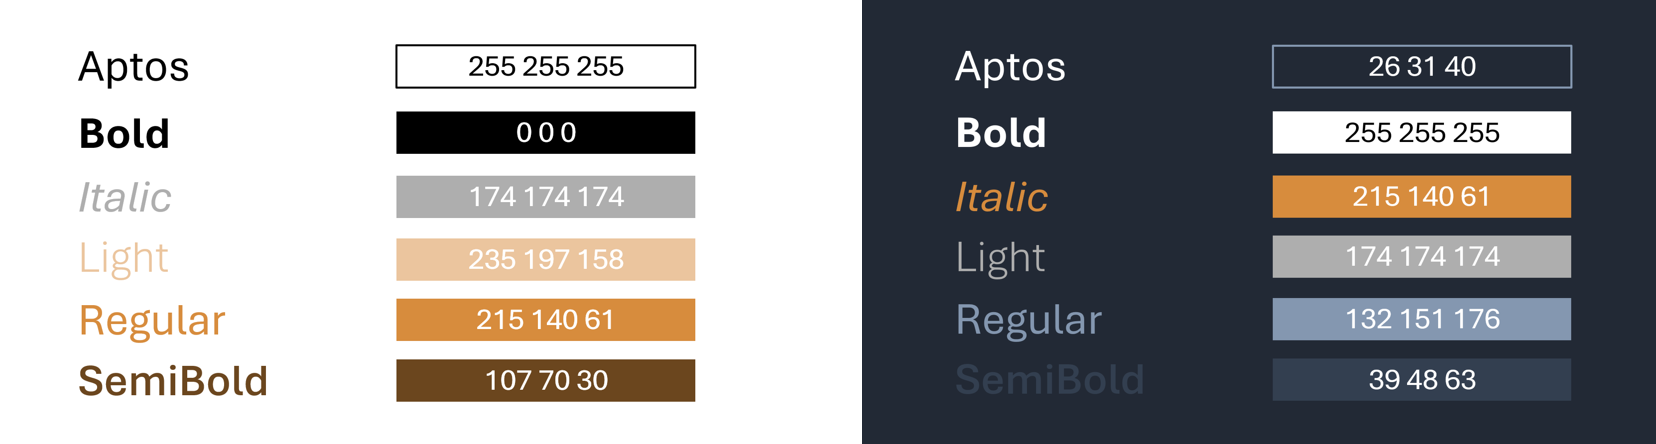
\includegraphics[clip,width=0.9\linewidth]{images/Farbpalette.png}
    \caption[Farbpalette für den Light Mode und Dark Mode]{Farbpalette für den Light Mode und Dark Mode}
    \label{Farbpalette}
\end{figure}

Die Farbpalette für den Light Mode besteht aus verschiedenen Orangetönen und einem Braun. Die Hintergrundfarbe des Dark Modes ist ein dunkles Blau, Orange wird nur noch als Akzentfarbe verwendet, ansonsten wird ein helleres Blau genutzt.
Die Schriftart "Aptos" wurde aufgrund ihrer Lesbarkeit und Ästhetik ausgewählt.

Ein zentrales Element des UX Designs war die Entwicklung eines klaren und intuitiven Bedienungskonzepts. Ziel war es, eine benutzerfreundliche Navigation zu schaffen, die es den Nutzern ermöglicht, alle Funktionen der Anwendung schnell und einfach zu erreichen.

\begin{figure}[h]
    \centering
    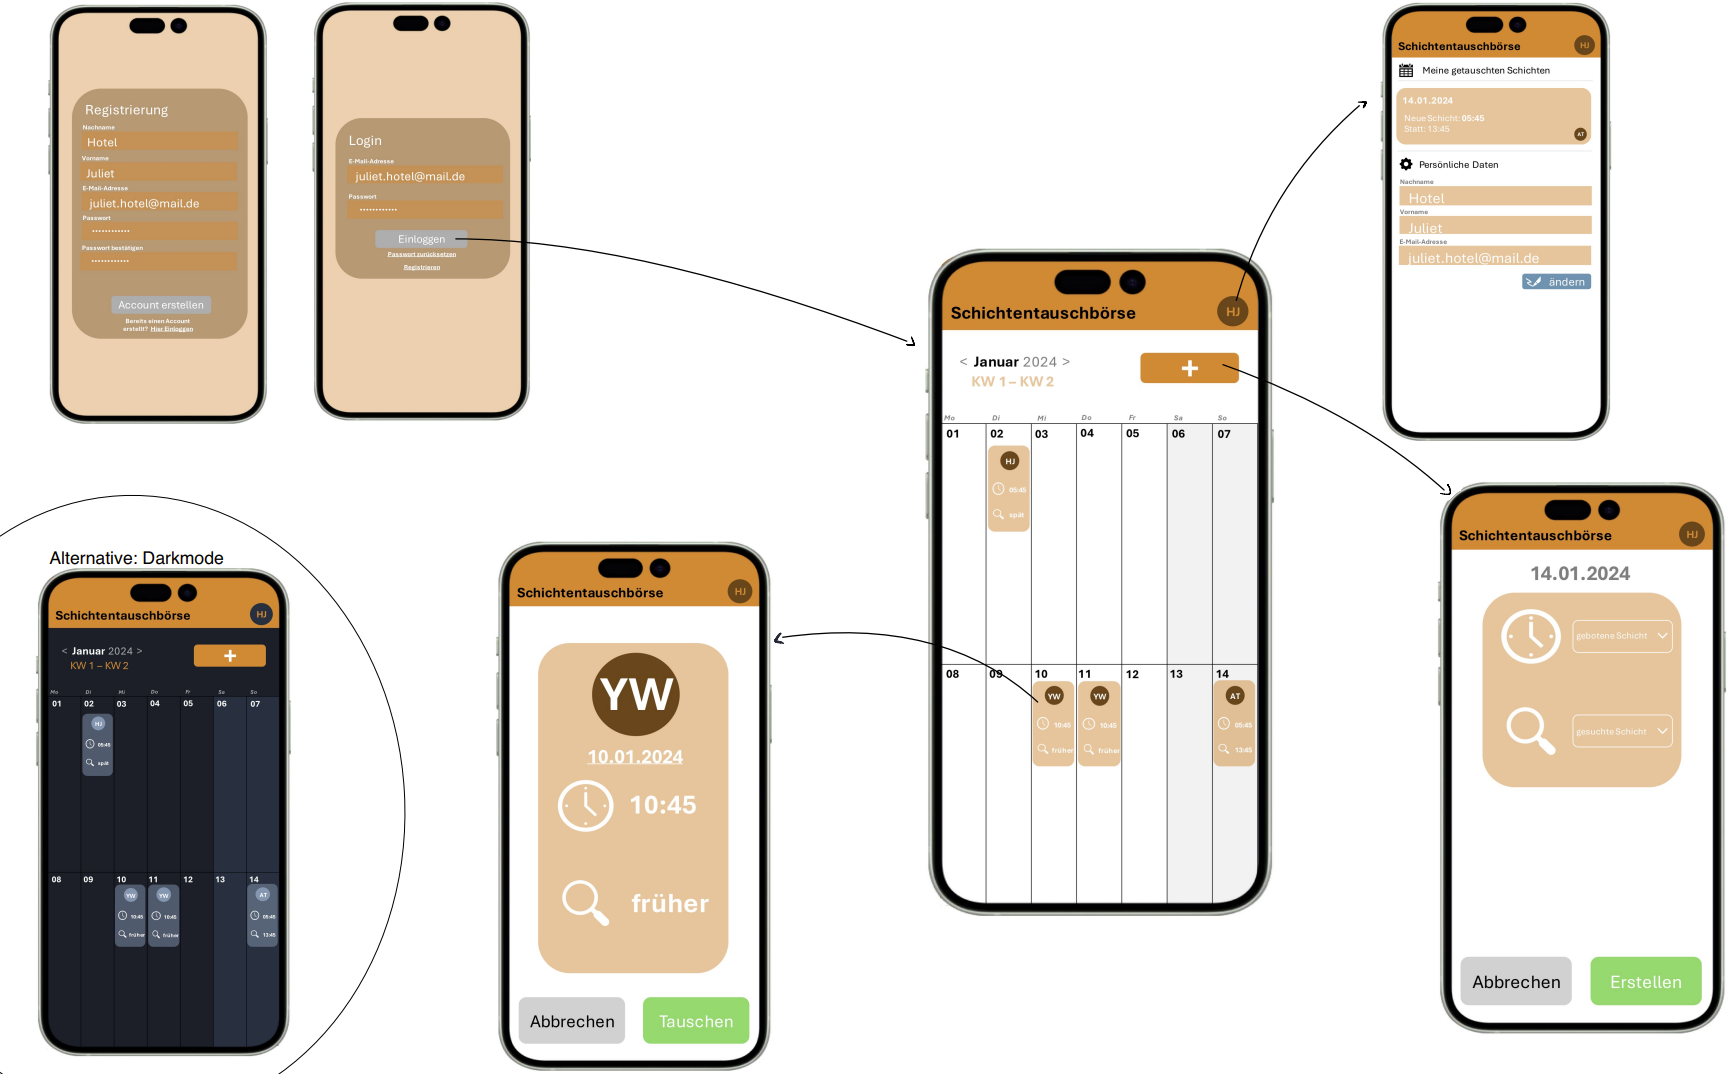
\includegraphics[clip,width=0.9\linewidth]{images/Bedienungskonzept_V1.png}
    \caption[Bedienungskonzept der Anwendung]{Bedienungskonzept der Anwendung}
    \label{Bedienungskonzept_V1}
\end{figure}

Nachdem sich der Nutzer registriert und anschließend erfolgreich angemeldet hat, gelangt er auf die zentrale Übersichtsseite, wie in Abbildung \ref{Bedienungskonzept_V1} dargestellt. 
Diese ermöglicht den Zugang zu allen anderen Seiten der Anwendung. 
Über die User-Kennung im Header gelangt der Nutzer zu einer Einstellungsseite. 
Dort kann er seine persönlichen Daten ändern und die bereits getauschten Schichten einsehen. 
Durch Klicken auf den Namen der Anwendung "Schichtentauschbörse" im Header gelangt er jederzeit zurück zur Übersicht.

Möchte ein Nutzer eine neue Tauschanfrage erstellen, ist das über den Button direkt unter dem Header möglich. 
Dabei wird eine neue Seite aufgerufen, auf der die gebotene und gesuchte Schicht aus einem Dropdown-Menü ausgewählt werden können. 
Alternativ kann der Nutzer auch eine bestimmte Uhrzeit eingeben, falls eine spezifische Zeit gewünscht ist. 
Wenn der Nutzer seine Anfrage doch nicht stellen möchte, kann er den Vorgang abbrechen und gelangt zurück zur Übersichtsseite. 
Mit dem Drücken des „Erstellen“-Buttons wird die neue Tauschanfrage finalisiert und im Kalender für alle Nutzer sichtbar.

Klickt ein Nutzer im Kalender auf eine Anfrage, kann er das Annehmen der Tauschanfrage entweder über den Button „Abbrechen“ beenden oder über den Button „Tauschen“ die Schicht tauschen. 
Nach dem Annehmen verschwindet die Tauschanfrage aus dem Kalender und wird in den Einstellungen unter „Meine getauschten Schichten“ angezeigt.

Zusätzlich wurde eine alternative Dark Mode-Version der Übersichtsseite erstellt, um unterschiedliche Präferenzen der Nutzer einzubinden.

\section{Phase 5: Nutzerumfrage}
\label{chap:nutzerumfrage}
\subsection{Methodik und Durchführung der Nutzerumfrage}

\subsection{Auswertung und Analyse der Nutzerumfrage}